% For each digit length L
\subsubsection{ Counter write }
% For each index in 1, 2, 3, and carry in 0,1

\begin{itemize}

    \item For each $i = 1,2,3$,
                   $j = l-1,\ldots,1$,
                   $u \in \{0, 1\}^j$, and each
                   $\inc \in \{{\tt increment}, {\tt copy} \}$:
        \begin{itemize}
        \item Create
        $\begin{aligned}[t]
            \cwrite(& \left\langle {\tt Write}, i, u0, \inc \right\rangle,
                       \left\langle {\tt Write}, i, u,  \inc \right\rangle \;)
        \end{aligned}$ \\ from the general gadget in Figure~\ref{fig:counter_write_0}

        \item Create
        $\begin{aligned}[t]
            \cwrite(& \left\langle {\tt Write}, i,  u1, \inc \right\rangle,
                       \left\langle {\tt Write}, i,  u,  \inc \right\rangle \;)
        \end{aligned}$ \\ from the general gadget in Figure~\ref{fig:counter_write_1}


        \item Create
        $\begin{aligned}[t]
            \cwrite(& \left\langle {\tt Write}, 1, u0, \inc, {\tt msr} \right\rangle,
                       \left\langle {\tt Write}, 1, u,  \inc, {\tt msr} \right\rangle \;)
        \end{aligned}$ \\ from the general gadget in Figure~\ref{fig:counter_write_0}

        \item Create
        $\begin{aligned}[t]
            \cwrite(& \left\langle {\tt Write}, 1,  u1, \inc, {\tt msr} \right\rangle,
                       \left\langle {\tt Write}, 1,  u,  \inc, {\tt msr} \right\rangle \;)
        \end{aligned}$ \\ from the general gadget in Figure~\ref{fig:counter_write_1}

        \item Create
        $\begin{aligned}[t]
            \cwrite(& \left\langle {\tt Write}, i, u0, \inc, {\tt msr}, {\tt msd} \right\rangle,
                       \left\langle {\tt Write}, i, u,  \inc, {\tt msr}, {\tt msd} \right\rangle \;)
        \end{aligned}$ \\ from the general gadget in Figure~\ref{fig:counter_write_0}

        \item Create
        $\begin{aligned}[t]
            \cwrite(& \left\langle {\tt Write}, i,  u1, \inc, {\tt msr}, {\tt msd}\right\rangle,
                       \left\langle {\tt Write}, i,  u,  \inc, {\tt msr}, {\tt msd}\right\rangle \;)
        \end{aligned}$ \\ from the general gadget in Figure~\ref{fig:counter_write_1}
        \end{itemize}

    \item For each $i = 1,2,3$ and each $\inc \in \{{\tt increment}, {\tt copy} \}$:
    \begin{itemize}
        \item Create
        $\begin{aligned}[t]
            \cwrite(& \left\langle {\tt Write},    i, 0, \inc \right\rangle,
                       \left\langle {\tt DigitTop}, i,    \inc \right\rangle \;)
        \end{aligned}$ \\ from the general gadget in Figure~\ref{fig:counter_write_0}

        \item Create
        $\begin{aligned}[t]
            \cwrite(& \left\langle {\tt Write},    i, 1, \inc \right\rangle,
                       \left\langle {\tt DigitTop}, i,    \inc \right\rangle \;)
        \end{aligned}$ \\ from the general gadget in Figure~\ref{fig:counter_write_1}

        \item Create
        $\begin{aligned}[t]
            \cwrite(& \left\langle {\tt Write},    1, 0, \inc, {\tt msr} \right\rangle,
                       \left\langle {\tt DigitTop}, 1,    \inc, {\tt msr} \right\rangle \;)
        \end{aligned}$ \\ from the general gadget in Figure~\ref{fig:counter_write_0}

        \item Create
        $\begin{aligned}[t]
            \cwrite(& \left\langle {\tt Write},    1, 1, \inc, {\tt msr} \right\rangle,
                       \left\langle {\tt DigitTop}, 1,    \inc, {\tt msr} \right\rangle \;)
        \end{aligned}$ \\ from the general gadget in Figure~\ref{fig:counter_write_1}

        \item Create
        $\begin{aligned}[t]
            \cwrite(& \left\langle {\tt Write},    i, 0, \inc, {\tt msr}, {\tt msd}\right\rangle,
                       \left\langle {\tt DigitTop}, i,    \inc, {\tt msr}, {\tt msd}\right\rangle \;)
        \end{aligned}$ \\ from the general gadget in Figure~\ref{fig:counter_write_0}

        \item Create
        $\begin{aligned}[t]
            \cwrite(& \left\langle {\tt Write},    i, 1, \inc, {\tt msr}, {\tt msd}\right\rangle,
                       \left\langle {\tt DigitTop}, i,    \inc, {\tt msr}, {\tt msd}\right\rangle \;)
        \end{aligned}$ \\ from the general gadget in Figure~\ref{fig:counter_write_1}
    \end{itemize}

\end{itemize}

\vspace{.5cm}

\begin{figure}[H]
    \centering
    \begin{subfigure}[t]{0.2\textwidth}
        \centering
        
\includegraphics[width=0.2\textwidth]{counter_write_0}
        \caption{\label{fig:counter_write_0} {\tt Counter\_Write\_0}}
    \end{subfigure}%
    ~
    \begin{subfigure}[t]{0.2\textwidth}
        \centering
        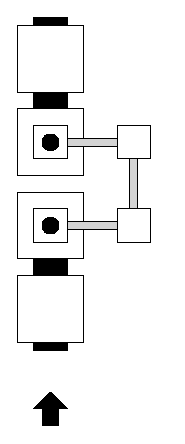
\includegraphics[width=0.2\textwidth]{counter_write_1}
        \caption{\label{fig:counter_write_1} {\tt Counter\_Write\_1}}
    \end{subfigure}%
    \caption{\label{fig:counter_write} The {\tt Counter\_Write} gadgets}
\end{figure}